\chapter{Background}

Malware is a malicious program intended to do pernicious exercises on a client's computer with the proposition of removing data and misusing assets without his assent. Viruses and worms, are the best known types of malware on account of the way in which they spread, instead of their behavior. Malware is now and then utilized widely against government or corporate websites to gather protected data or to disturb their operations by large. Also, malware is regularly utilized against people to steal data, for example, personal identification numbers or bank or credit card details and passwords. As per a survey on data breaches led by Verizon in 2014, culprits considered Citadel as the preferred banking malware to theft individual information, while Zeus keeps on being the favorite banking malware for stealing money from bank accounts [9].

Figure 1 shows how the malware is swiftly growing in volume day-byday. In Figure 1, the x-axis specifies the year and the y-axis indicates the number of malware samples generated in the specified year on the x-axis.

\begin{figure}
    \centering    
    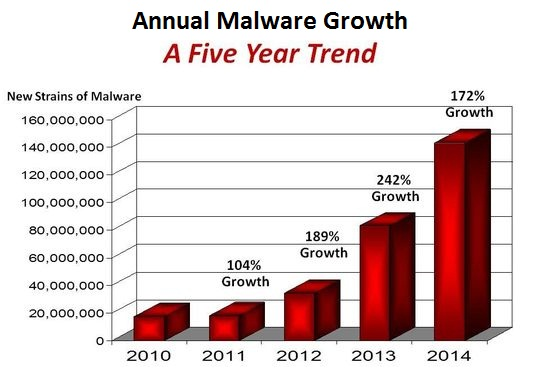
\includegraphics[width=8.4cm, height=6cm]{malware-growth-chart.jpg}
    \caption[Annual Malware Growth]{Annual Malware Growth [10]}
\end{figure}
Virus writers are aware that signature-based detection with heuristic analysis can be the basis of modern malware detection techniques. So, virus developers have created numerous procedures and techniques to evade signature-based detection. In January 2015, AV-TEST's CEO said, "Many of the new malware samples are just variants of existing viruses. They have been modified so that they are no more identified and thus, AV signature updates are required" [10]. Some of the noteworthy techniques used by virus writers to evade signature detection are encryption, polymorphism and metamorphism.

\section{Encrypted Malware} 

Cascade virus, which initially appeared in late 1986, was the first malware that used encryption strategy to scramble its contents [11]. Cascade virus comprises of two parts. First part is a decryptor and the second part is encrypted malware code. The reason for encryption is to conceal the malware signature, to evade signature identification. Later, this technique was adopted by almost every encrypted malware.  For the most part, virus writers use extremely simple and weak encryption methods, for example, a repeated XOR with a fixed bit pattern. Cascade malware also used XOR operation as encryption routine because of its symmetrical and reversible feature. In the event that the encryption key of malware was changed after every infection, the encrypted body signature also gets changed. If in case the same decryptor was used, signature detection technique can make use of decryptor code signature to detect the malware.
\begin{figure}
    \centering    
    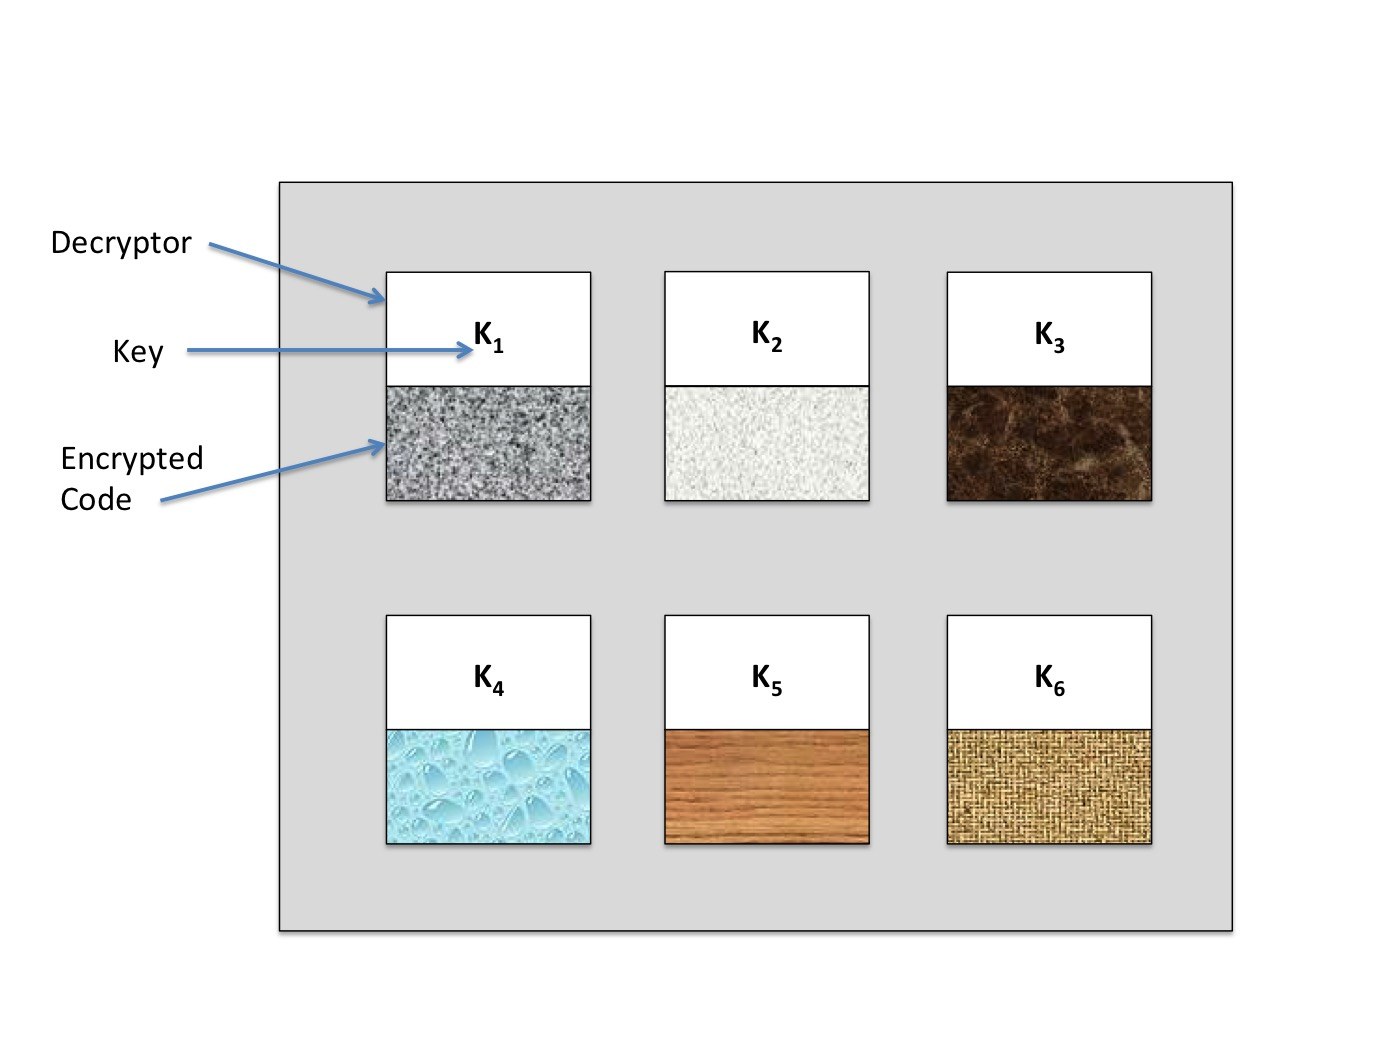
\includegraphics[width=8cm, height=6cm]{encryptedvirus.jpg}
    \caption[Encrypted Malware Replication]{An Encrypting Malware spreads without changing decryptor but the key within decryptor varies from infection to infection. As the key value changes, the encrypted virus body also changes [14].}
\end{figure}
\section{Polymorphic Malware} 

Similar to an encrypted malware, polymorphic malware incorporates an encrypted virus code and a decryptor. Additionally in a polymorphic virus, the decryptor is morphed. During polymorphic malware propogation, not only is the virus code encrypted, but the decryptor also varies from infection to infection. As there is no fixed signature or no fixed decryptor to scan for, no two infections look alike to be exploited by the antivirus program for detection purpose [16]. Polymorphic virus uses code obfuscation techniques, for example, including junk codes or substitution of instructions, to mutate its decryptor [18].
Several techniques are utilized to decrypt the polymorphic virus, such as, cryptanalysis (also called x-ray), emulation and dedicated decryption routines [21].

\begin{figure}
  \centering
\begin{lstlisting}[language=myasm]
MOV A,R$1$        MOV A,R$1$        MOV A,R$1$        MOV A,R$1$        MOV A,R$1$
ADD B,R$1$        NOP             ADD #0,R$1$       OR R$1$,R$1$        TST R$1$
ADD C,R$1$        ADD B,R$1$        ADD B,R$1$        ADD B,R$1$        ADD C,R$1$
SUB #4,R$1$       NOP             OR R$1$,R$1$        MOV R$1$,R$5$       MOV R$1$,R$5$
MOV R$1$,X        ADD C,R$1$        ADD C,R$1$        ADD C,R$1$        ADD B,R$1$
                NOP             SHL #0,R$1$       SHL R$1$,0        CMP R$2$,R$5$
                SUB #4,R$1$       SUB #4,R$1$       SUB #4,R$1$       SUB #4,R$1$
                NOP             JMP .+1         ADD R$5$,R$5$       JMP .+1
                MOV R$1$,X        MOV R$1$,X        MOV R$1$,X        MOV R$1$,X
                                                MOV R$5$,Y        MOV R$5$,Y
(a)             (b)             (c)             (d)             (e)


\end{lstlisting}
    \caption[Examples of a polymorphic virus.]{Examples of a polymorphic virus utilizing code obfuscation techniques. All of the Figure~\ref{fig:polyvirus} snippets perform the same operation, i.e.,  X = (A + B + C - 4). For instance, the program snippet of Figure~\ref{fig:polyvirus} (c) is functionally the same as Figure~\ref{fig:polyvirus} (a) in light of the fact that instructions like adding 0 to a register, ORing R1 with itself, shifting R1 left 0 bits, and jumping to the next instruction all do nothing [19].}
    \label{fig:polyvirus}
\end{figure}

    
The first polymorphic malware, 1260, was developed by Mark Washburn in 1990 [15]. And the first widespread polymorphic infection was caused by Tequila and Maltese Amoeba virus, in 1991 [16].

\section{Metamorphic Malware} 

Virus writers took the next step and developed an advanced variant of polymorphic malware, known as Metamorphic malware. Generally, before infection, polymorphic malware encrypt the virus code and morph the decryptor, while metamorphic malware morph the whole virus code. According to Igor Muttik, "Metamorphics are bodypolymorphics", since polymorphism is applied to the entire virus body [22]. Metamorphic viruses utilizes several code morphing techniques that constitue instruction reordering, data reordering, subroutine inlining, subroutine outlining, register renaming, code permutation, instruction substitution and garbage code insertion [23]. Figure~\ref{fig:aimalware} illustrates the metamorphic malware with different signatures.

\begin{figure}
  \centering
      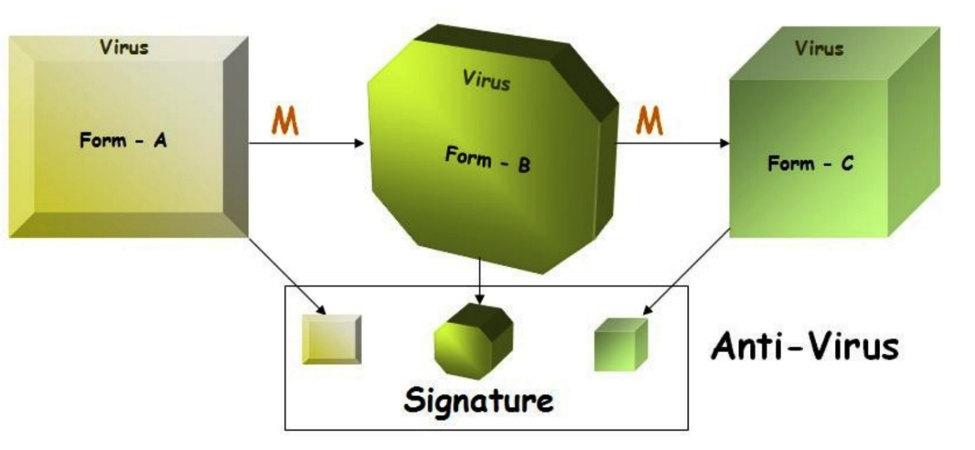
\includegraphics[width=9cm, height=4.5cm]{aimalwarepic.png}
    \caption[Metamorphic malware with different signatures]{Metamorphic malware with different signatures [20].}
    \label{fig:aimalware}
\end{figure}

\subsection{Register renaming} 

In December 1998, a metamorphic malware named Win95/Regswap was developed by Vecna [22]. Regswap used register renaming technique to morph the virus code. In this technique, instructions gets modified to use different registers. As just the register operands gets altered that too in some part of the code instead of whole code, so the complexity of final modified code wouldn't be high. Figure~\ref{fig:regswap} depicts how the register renaming technique transforms the code.

\begin{figure}
  \centering
      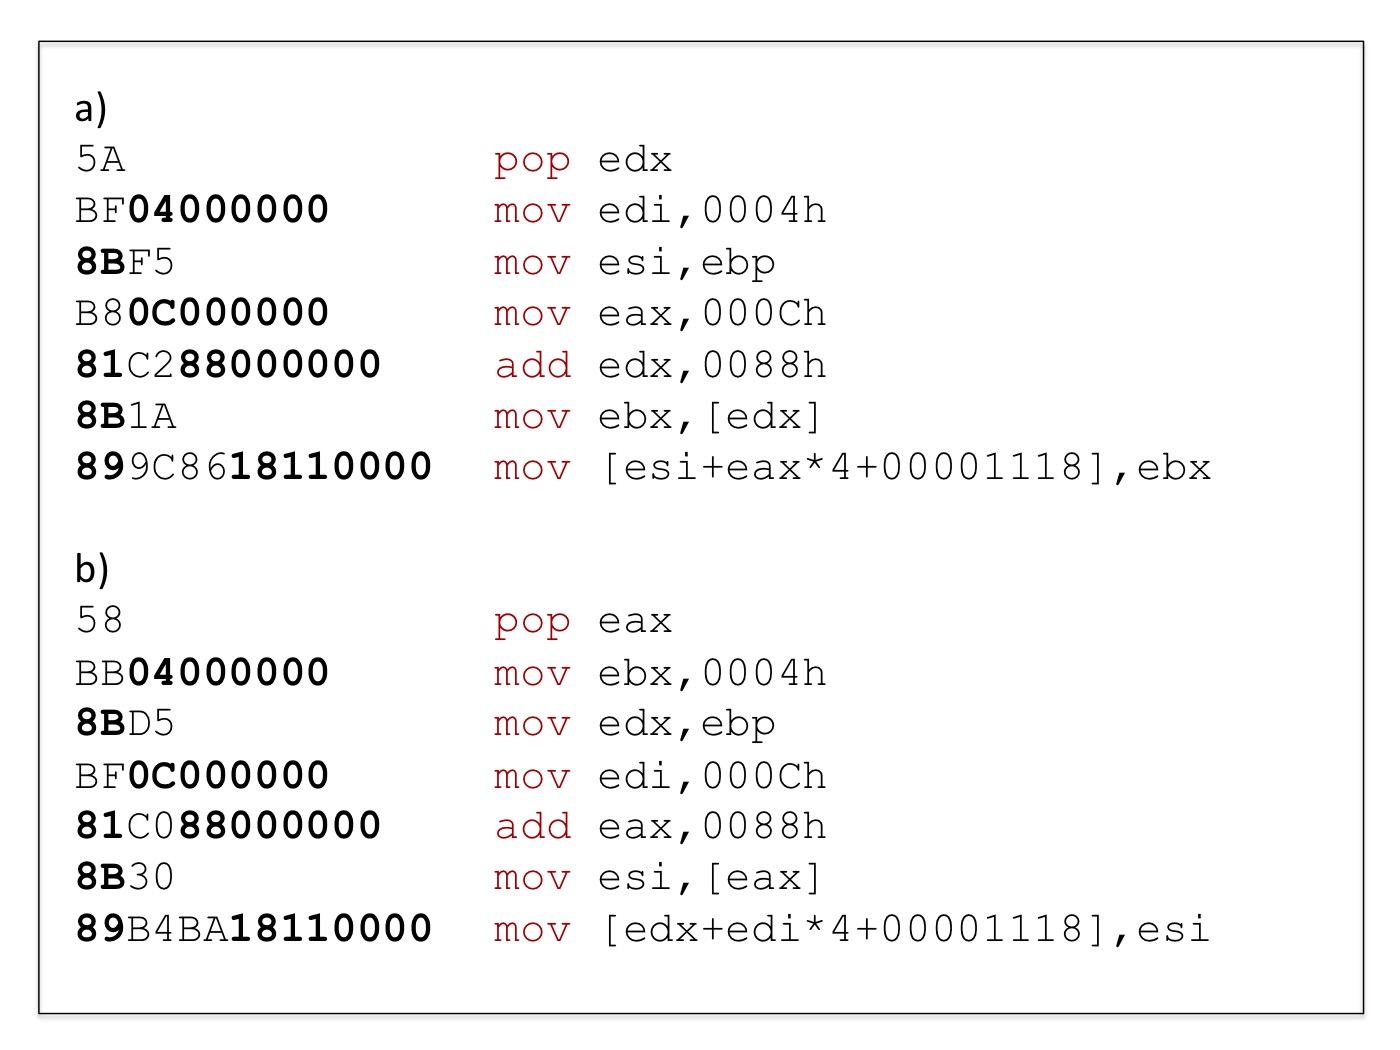
\includegraphics[width=12.9cm, height=9cm]{regswap.jpg}
    \caption[Register Renaming Example]{code snippet extracted from two different versions of RegSwap [22].}
    \label{fig:regswap}
\end{figure}

The bold areas in figure~\ref{fig:regswap} illustrates the similarities of the two different code versions. Thus, a wildcard string, such as 5? B?, could be useful to detect the malware code [22]. 

\subsection{Dead code insertion} 

Dead code can be a single instruction or a block of instructions, for example, adding NOPs [23], adding 0 to a register, moving between same registers, ORing register with itself, shifting register left 0 bits, jumping to next instruction, incrementing a register immediately followed by decrementing the same register by same value. Inserting dead code or do-nothing instructions is the easiest approach to morph the virus code without modifying its functionality [23]. 
The Win32/Evol virus, which was found around July 2000 [24], used dead code insertion approach to obfuscate the signature of a code as illustrated in Figure~\ref{fig:deadcode}. 

\begin{figure}
  \centering
  \begin{lstlisting}[language=myasm]
C$7060$F$000055$				MOV [esi], $5500000$Fh
C$746048$BEC$5151$		MOV [esi+0004], $5151$EC$8$Bh
BF$0$F$00055$					MOV edi, $5500000$Fh
$893$E 						MOV [esi], edi
$5$F 						POP edi						; garbage
52 					PUSH edx						; garbage
B$640$ 						MOV dh, 40 					; garbage
BA$8$BEC$5151$ 				MOV edx, $5151$EC$8$Bh
53 					PUSH ebx						; garbage
$8$BDA					MOV ebx, edx
$895$E$04$						MOV [esi+0004], ebx  
\end{lstlisting}
    \caption[Example of code metamorphosis of Evol virus ]{Example of code metamorphosis of Evol virus with Dead code insertion [23].}
    \label{fig:deadcode}
\end{figure}

\subsection{Subroutine permutation} 

Code may contain several subroutines (or) functions and changing the order of this subroutines may not impact the execution of code. Subroutine permutation approach makes use of this advantage i.e., altering the order of subroutines, to change its internal structure without modifying the functionality of code. A code with n different subroutines can generate n! different permutations of subroutines, thus large number of versions of the same code can be generated [4].

\begin{figure}
  \centering
      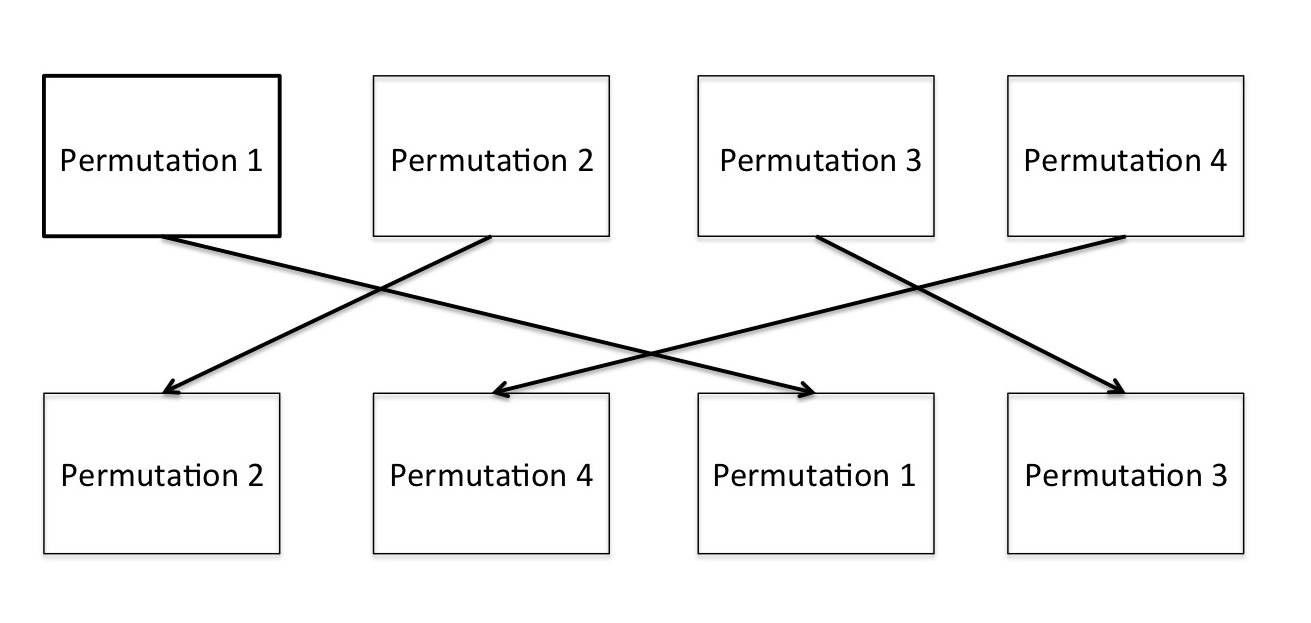
\includegraphics[width=12cm, height=6cm]{subpermutation.jpg}
    \caption[Example of subroutines permutation]{Example of subroutines permutation [23].}
    \label{fig:subpermutation}
\end{figure}

\section{Transcriptase}

Typesetting text is generally pretty easy. However, there are some special
characters that will not be typeset as you might expect. In the remainder of this
section we consider some of the most common of these
special characters. 

The backslash ``\verb+\+'' is used 
as the ``escape'' character, meaning that
whatever follows a backslash is interpreted as a macro.
For example, when \verb+\LaTeX+ is typeset, it looks like \LaTeX, which 
is a lot different from LaTeX.

To get double quotes, use two single quotes. That is, the left double quote is ``, while the right double
quote is ''. When you do it correctly, quoted text looks ``like this.''
If you use the double quote key, you will always get right-quotes, which looks "like this," and is
almost certainly not what you want.

A tilde ``\verb+~+'' is used as a ``tie,'' that is, a space is inserted, but no line break can occur.
For example, you might type Dr.~Stamp just to be sure that the line of text
does not break between Dr. and Stamp, as it otherwise might.

The percent sign is used for comments---everything following a percent sign 
on a given line is ignored when you \LaTeX\ your file. % Like this stuff here
If you want a percent sign to appear in your document, use \verb+\%+, 
which will give you this \%.

The dollar sign also has special meaning, since it is used to start and end
math formulas. To typeset a dollar sign, use \verb+\$+, like this~\$.

To force \LaTeX\ to insert a space, use a backslash followed by
a space, that is, \verb+\ +. You can put in multiple extra spaces\ \ \ \ \ \ \ if you want.

\section{Rhino}

To change fonts, enclose the text in curly brackets and give the appropriate font command.
For example, to italicize text, {\it do this}, and to get boldface, {\bf this is the ticket}.
Another useful font is {\tt this one}, which produces a typewriter-like font.

